\section{Generierung von Testdaten}

\textbf{Aus FORUM Artikel}

Um das Testen von Datenbank-basierten Anwendungen zu erleichtern, soll es möglich sein, automatisch Testdaten für funktionale Tests aus dem Datenbankschema generieren zu lassen. Die generierten Testdaten können direkt bzw. als Basis für die Erstellung von Testdatensätzen genutzt werden (vgl. Abb. 3). 

Bei der Testdatengenerierung sind u.a. folgende Anforderungen zu berücksichtigen:

\begin{itemize}

\item Die Testdaten müssen dem Datenbankschema der Anwendung entsprechen, um diese Daten überhaupt in die Datenbank einspielen zu können.
\item Die Testdaten sollen einerseits genügend Daten enthalten, um die fachliche Struktur der Anwendungsdaten zu erhalten; andererseits sollen möglichst wenige Daten erzeugt werden, damit die eingespielten Daten übersichtlich und für die Software-Tester verständlich bleiben.
\item Für die Durchführung und Wartung von Tests ist es von Vorteil, wenn möglichst viele Tests dieselben Testdaten verwenden können, d.h. wenn die generierten Testdaten eine möglichst große Testabdeckung erzielen. Somit sind insgesamt weniger Testdatensätze zu verwalten, was z.B. bei Änderung des zugrundeliegenden Datenbankschemas von Vorteil ist und die Übersichtlichkeit erhöht.
\item Die Beschreibung des Datenbankschemas, aus dem die Testdaten generiert werden, muss so ausdrucksmächtig sein, dass auch Sachverhalte beschrieben werden können, die über die strukturelle Abbildung, z.B. auf Datenbank-Tabellen, hinausgehen, damit die Testdaten auch den weitergehenden Anforderungen des Systems under Test genügen und realistische Szenarien abbilden. Beispielsweise kann eine Anwendung eine 1<->1..* Beziehung definieren; in einem relationalen Datenbanksystem ist jedoch nur eine 1<->0..* Beziehung durch Fremdschlüssel- und Not-Null-Constraints strukturell abbildbar.
\item Die generierten Daten sollen in der entwickelten DSL beschrieben werden, damit diese direkt im STU Test-Framework nutzbar sind.
\end{itemize}

Interessanterweise stellte sich bei einer umfassenden Literaturanalyse und Analyse existierender Testdatengeneratoren heraus, dass bisher keine passende Lösung für die beschriebene Problemstellung existiert. In der Wissenschaft beschriebene Ansätze und Algorithmen generieren meist für eine zu testende SQL-Abfrage einen passenden Testdatenbestand. Einer SQL-Abfrage liegt dabei eine formale Spezifikation zu Grunde, die allerdings für ein Anwendungsprogramm normalerweise nicht vorhanden ist. Existierende Software-Werkzeuge fokussieren sich auf die Generierung von Massendaten, die v.a. für Performanz-Tests und nicht für funktionale Tests geeignet sind. Dies zeigt sich auch daran, dass diese Werkzeuge Beziehungen zwischen Entitäten nur zufällig erzeugen und im Allgemeinen wesentlich mehr Daten generieren als für einen Menschen noch einfach verständlich sind. Weiterhin deuten Untersuchungen im Projekt darauf hin, dass die Komplexität der Testdatengenerierung im allgemeinen Fall nicht-polynomial ist.

Aus diesem Grund wurde ein neuer, effizienter Algorithmus zur Testdatengenerierung für die Projektproblemstellung entworfen. Anleihen konnten dabei aus [5] gezogen werden. Der entwickelte Algorithmus berücksichtigt lokal alle Kombinationen der unteren und oberen Grenzwerte von binären Beziehungstypen n..N<->m..M und versucht gleichzeitig die Anzahl der generierten Entitäten und Beziehungen zu minimieren. Globale, d.h. "transitive" Abhängigkeiten über mehrere Beziehungstypen hinweg, die zu einer kombinatorischen Explosion führen können, bleiben dabei (augenblicklich) unberücksichtigt. Weitere Details zu dem im Projekt entwickelten Verfahren zur Testdatengenerierung (u.a. Beschreibung des Algorithmus in Pseudo-Code) sind [6] zu entnehmen.

%Der entwickelte Testdatengenerator wurde auf ein Datenbankschema eines produktiven Anwendungssystems mit 12 Datenbanktabellen und einigen fachlichen Einschränkungen angewendet. Durch unser Verfahren zur Testdatengenerierung wurde ein konsistenter, übersichtlicher Satz an Testdaten erzeugt, der eine gute Startbasis für Anwendungstest bietet.
%
%Der Code des DSL-Interpreters und des Testdatengenerators ist verfügbar unter https://github.com/Seitenbau/stu/.



\textbf{Outline}

% Idee hinter dem Algorithmus


	\subsection{Beschreibung des Algorithmus}
	
	Generieren der Beziehungen

  Der Algorithmus betrachtet das Datenbank-Schema als Graph. Die Tabellen stellen die Knoten und die Beziehungen stellen die Kanten dar.
  Da assoziative Tabellen ebenfalls Beziehungen ausdrücken, werden diese vom Algorithmus als besondere Kante behandelt. Der Graph wird
	ausgehend von eines Knotens traversiert. Alle Kanten des aktuellen Knotens und die damit verbundenen Knoten werden rekursiv besucht.
	Der Algorithmus erzeugt zu jeder Kante Entitäten der beiden beteiligten Tabellen. % hier evtl die Grenzfälle erläutern...
	Jede Kante und jede Tabelle werden genau genau einmal durchlaufen.
	
  Der Algorithmus soll an dem in Abb.~\ref{database} dargestellten Datenbank-Schema einer Bücherverwaltung veranschaulicht werden. Ein
	Buch gehört genau zu einem Verlag und wird von beliebig vielen (mindestens einer) Autoren geschrieben. Ein Verlag kann selbst beliebig
	viele und sogar keine Bücher veröffentlichen und ein Autor kann an keinem oder beliebig Büchern beteiligt sein.
	
	\begin{figure}[htb]
		\begin{center}
			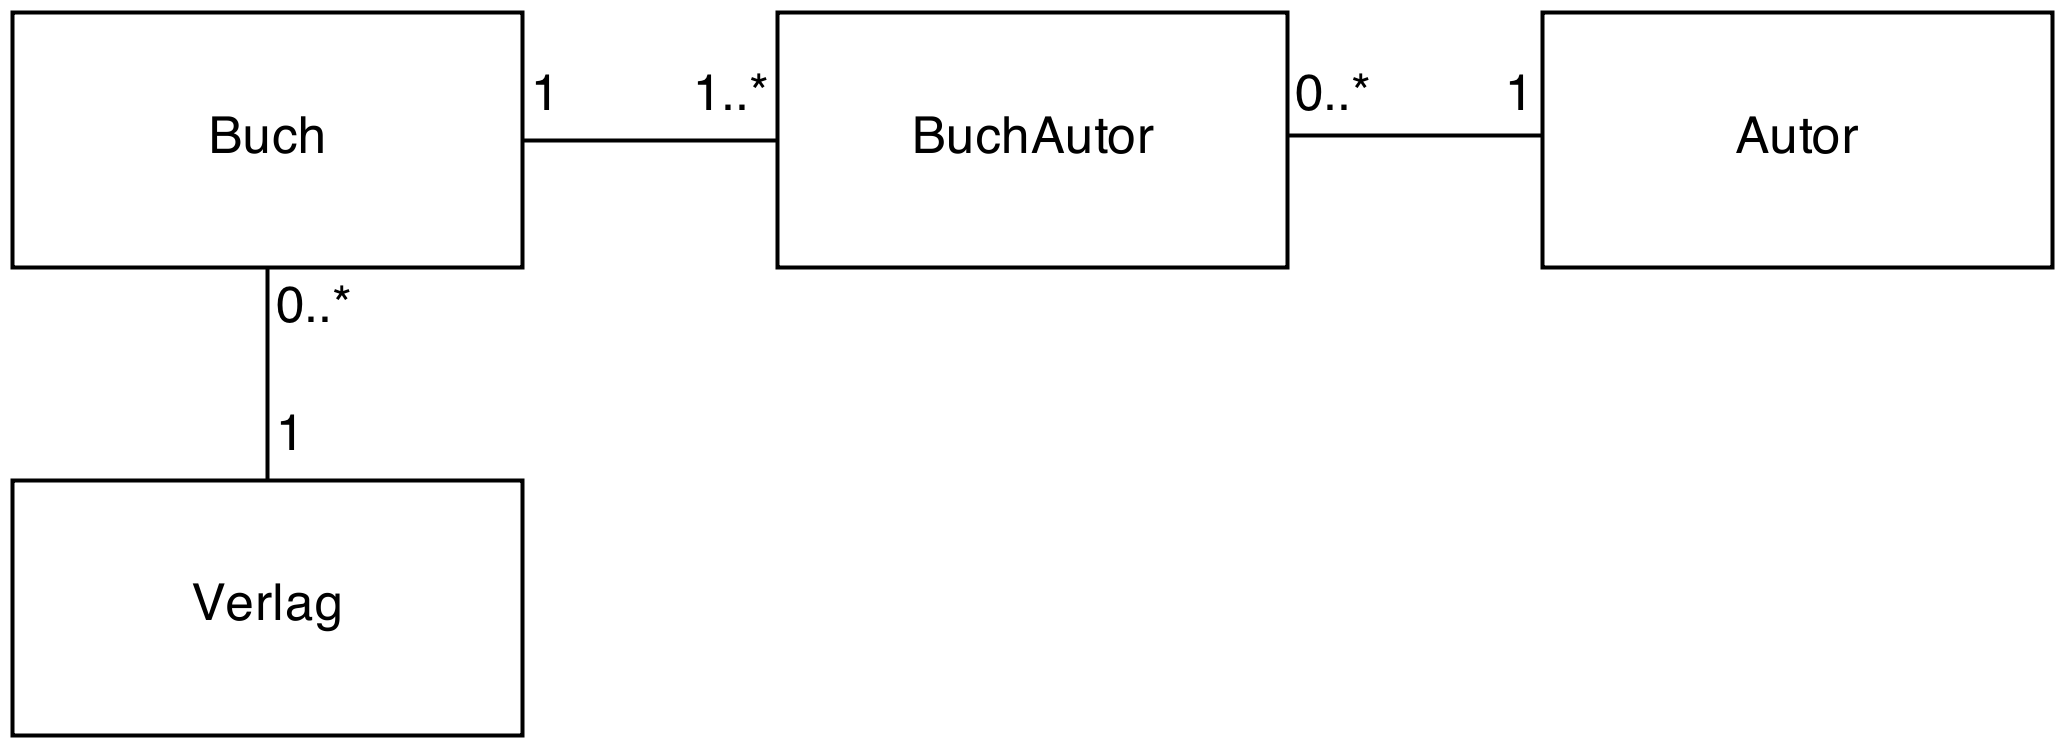
\includegraphics[width=8cm]{images/database.png}
			\caption{\label{database}Datenbank-Schema der Bücherverwaltung}
		\end{center}
	\end{figure}
	
	Als Ausgangspunkt für die Traversierung wird der Knoten Buch verwendet. Von diesem Knoten aus werden alle Kanten besucht, angefangen mit
	der Kante zum Knoten Verlag. Dieser repräsentiert eine 1:0..*-Beziehung. Um möglichst alle Grenzfälle abzudecken, wird eine Entität
	von Verlag erzeugt, die keine Bücher verlegt. Außerdem wird ein Verlag generiert, der genau ein Buch verlegt, und ein Verlag, der viele
	Bücher veröffentlicht. Anstelle von * kann ein konfigurierbarer Wert verwendet werden, in dem Beispiel wird dafür $4$ verwendet. Für
	diese Kante werden also drei Entitäten des Typs Verlag und fünf Entitäten des Typs Buch erzeugt.
	
  Der Knoten Verlag hat keine nicht-besuchten Kanten, weshalb die Traversierung in Buch fortgesetzt wird mit der Kante zum Knoten
	BuchAutor. Die Kante hat eine assoziative Tabelle als Ziel, weshalb hier andere Schritte notwendig sind wie bei der letzten Kante.
	Die Tabelle BuchAutor drückt eine 0..*:1..*-Beziehung zwischen Buch und Autor aus. Der Algorithmus sieht vor, die vier möglichen
	min/max-Kombinationen generiert werden. Jede Beziehung zwischen einem Buch und einem Autor führt zu einer Entität in der Tabelle
	BuchAutor. Es wird ein Autor benötigt, der kein Buch geschrieben hat, und ein Autor, der genau an einem
	Buch beteiligt ist (min:min). Außerdem wird ein Autor benötigt, der vier Bücher schreibt (max:min), und ein Buch, das vier Autoren
	hat (min:max). Und schließlich werden vier Bücher benötigt, die jeweils die gleichen vier Autoren haben (max:max). Für die assoziative
	Tabelle BuchAutor werden folglich zehn Entitäten des Typs Buch und elf Entitäten des Typs Autor benötigt, wobei die bereits erzeugten
	Entitäten des Typs Buch hier weiterverwendet werden. Die Traversierung endet hier, da jede Kante besucht wurde.
	
	Die fünf im vorausgegangenen Schritt erzeugten Entitäten des Typs Buch sind allerdings noch ungültig, da sie noch nicht zu einem Verlag
	gehören. Solche Entitäten werden im letzten Schritt behandelt. Alle Entitäten werden auf Gültigkeit bzgl. ihrer Beziehungen überprüft,
	und bei Bedarf werden weitere Beziehungen und falls notwendig weitere Entitäten erzeugt.
	

	\subsection{Implementierung und Evaluation}
	

